% -*- mode: latex; -*- mustache tags:  
\documentclass[10pt,twoside,english]{_support/latex/sbabook/sbabook}
\let\wholebook=\relax

\usepackage{import}
\subimport{_support/latex/}{common.tex}

%=================================================================
% Debug packages for page layout and overfull lines
% Remove the showtrims document option before printing
\ifshowtrims
  \usepackage{showframe}
  \usepackage[color=magenta,width=5mm]{_support/latex/overcolored}
\fi


% =================================================================
\title{Object-Relational Persistence with Glorp}
\author{E. Maringolo, N. Pratt and R. Withney}
\series{The Pharo Technology Booklet Collection — edited by S. Ducasse}

\hypersetup{
  pdftitle = {Object-Relational Persistence with Glorp},
  pdfauthor = {E. Maringolo, N. Pratt and R. Withney},
  pdfkeywords = {persistence, database, object-relational mapping, Pharo, Smalltalk}
}


% =================================================================
\begin{document}

% Title page and colophon on verso
\maketitle
\pagestyle{titlingpage}
\thispagestyle{titlingpage} % \pagestyle does not work on the first one…

\cleartoverso
{\small

  Copyright 2017 by E. Maringolo, N. Pratt and R. Withney.

  The contents of this book are protected under the Creative Commons
  Attribution-ShareAlike 3.0 Unported license.

  You are \textbf{free}:
  \begin{itemize}
  \item to \textbf{Share}: to copy, distribute and transmit the work,
  \item to \textbf{Remix}: to adapt the work,
  \end{itemize}

  Under the following conditions:
  \begin{description}
  \item[Attribution.] You must attribute the work in the manner specified by the
    author or licensor (but not in any way that suggests that they endorse you
    or your use of the work).
  \item[Share Alike.] If you alter, transform, or build upon this work, you may
    distribute the resulting work only under the same, similar or a compatible
    license.
  \end{description}

  For any reuse or distribution, you must make clear to others the
  license terms of this work. The best way to do this is with a link to
  this web page: \\
  \url{http://creativecommons.org/licenses/by-sa/3.0/}

  Any of the above conditions can be waived if you get permission from
  the copyright holder. Nothing in this license impairs or restricts the
  author's moral rights.

  \begin{center}
    
\includegraphics[width=0.2\textwidth]{_support/latex/sbabook/CreativeCommons-BY-SA.pdf}
  \end{center}

  Your fair dealing and other rights are in no way affected by the
  above. This is a human-readable summary of the Legal Code (the full
  license): \\
  \url{http://creativecommons.org/licenses/by-sa/3.0/legalcode}

  \vfill

  % Publication info would go here (publisher, ISBN, cover design…)
  Layout and typography based on the \textcode{sbabook} \LaTeX{} class by Damien
  Pollet.
}


\frontmatter
\pagestyle{plain}

\tableofcontents*
\clearpage\listoffigures

\mainmatter


This document describes the Glorp object-relational mapper. By reading it, you will learn how to map your objects to a relational database. It presents step by step how to use Glorp and its basic and advanced concepts in a tutorial. At the end we include an Appendix that revisits relational database concepts.
We thank the authors of the previous Glorp tutorials R. Withney and N. Pratt for having granted us the right to use some of their material. This document has been written by E. Maringolo and edited by S. Ducasse.
\chapter{What is Glorp?}
Working in a live object environment such as Pharo is great. You can freely create your domain objects and compose them as you like. Sometimes those objects can be stored in a way that preserves the original design but in other cases you have to store your objects in a Relational Database Management System (a.k.a. \textit{RDBMS}). This requires you to flatten your object graph into relational tables managed by the RDBMS.

This process of mapping object to tables is called \textit{Object-Relational Mapping} (\textit{ORM}). It imposes certain constraints on the design of your object model to support persisting it in tables. Some models are easier to map onto tables than others, the difficulty lies in what is known as the \textit{\href{https://en.wikipedia.org/wiki/Object-relational_impedance_mismatch}{Object-Relational Impedance Mismatch}\footnote{\url{https://en.wikipedia.org/wiki/Object-relational_impedance_mismatch}}}.

To work with relational databases, Pharo provides a battle-tested ORM created at CampSmalltalk a decade ago and maintained since then. Its name is Glorp for \textit{Generic Lightweight Object-Relational Persistence}. It is usually called both GLORP (all caps, as an acronym), or Glorp (as a proper name).

Glorp is a full-featured ORM which offers a number of features to reduce the \textit{impedance} as much as possible. Amongst those features, you'll find some features saving you from writing SQL queries by hand, managing transactions that rollback the changes to the objects in your image or commit them to the database, writing simple and complex queries using plain Pharo syntax, and other features that we will cover in this introduction chapter and in the advanced topics chapter.
\chapter{Installation}\section{Database server}
Before installing Glorp you should already have installed the RDBMS of your choice on your machine or a reacheable server, it could be \href{http://postgresql.org}{PostgreSQL (http://postgresql.org)}\footnote{\url{http://postgresql.org}}, \href{http://dev.mysql.com/}{MySQL (http://dev.mysql.com/)}\footnote{\url{http://dev.mysql.com/}}, \href{http://sqlite.org}{SQLite (http://sqlite.org)}\footnote{\url{http://sqlite.org}}, or any other of your preference (as long it is supported). Hereafter we will refer to this RDBMS of your choice as the \textit{Platform}.
\section{Database drivers}
Along with your working installation of your RDBMS you should have installed in
your image the database drivers required to connect to the server.
\subsection{Native drivers}
With Native drivers the raw protocol is written in Smalltalk and it uses Pharo
sockets to write and read the data from the wire. This has the advantage of
being self contained, because you don't depend on an external file or setup
to connect to a server. Also, because everything is written in Smalltalk
it is debuggable using Pharo tools down to a very low-level.
\subsection{Library wrapper drivers (FFI)}
Library Wrappers, as its name implies, wrap an underlying Operative System
shared library like a \textcode{.dll} or \textcode{.so}, these wrappers will access
the shared library functions by means of FFI
(\textit{Foreign Function Interface}) calls and data structures.

Using an external library enables you to use an official client implementation
of a proprietary protocol like Oracle, or you can be sure that even
if the protocol spec is open you can use the official version of it.
In order to use it in Pharo you need to implement the wrapper classes and methods.
\subsection{A common driver API}
There are plenty of drivers available in Pharo, however those drivers have
different API's making their use not directly interchangeable. Making it hard
to migrate to a different driver or to simultaneously support different RDBMS.

To solve that there is Garage (aka \textit{Garage Drivers}), that provides a common
API for the different driver implementations. Garage is Pharo's analogous to
ODBC, JDBC or ADO.NET drivers.

Using this common API your code won't need to change if, for example, you decide
to move from MySQL to PostgreSQL, as long as you don't use exclusive features,
because all the implemented drivers will conform to the common Garage API.


\begin{figure}

\begin{center}
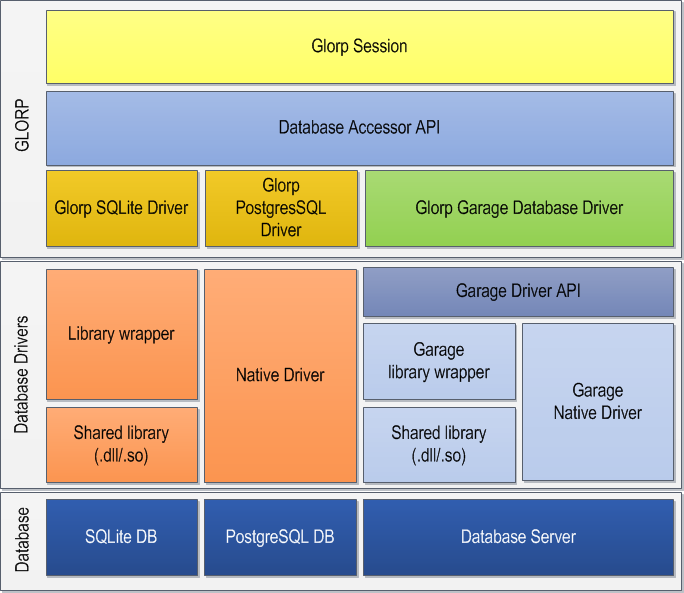
\includegraphics[width=0.72\textwidth]{/Users/ducasse/Workspace/FirstCircle/MyBooks/Bk-Writing/PharoBooks2/Booklet-Glorp/_result/pdf/Chapters/Glorp/figures/Glorp-UDBC.png}\caption{Connectivity parts\label{Garage diagram}}\end{center}
\end{figure}

\subsection{Available drivers}
There are many drivers available drivers in different versions of Pharo, as
the time of writing this, these are the currently supported drivers are:

\begin{itemize}
\item P3 (Native PostgreSQL v3 protocol)
\item Garage
\begin{itemize}
\item PostgreSQL (Native)
\item MySQL (Native)
\end{itemize}

\item UDBC SQLite3
\end{itemize}
\subsection{Glorp with P3}
P3 is a modern, lean and mean PostgreSQL client for Pharo.

P3Client uses frontend/backend protocol 3.0 (PostgreSQL version 7.4 {[}2003{]} and later), implementing the simple query cycle. It supports plaintext and md5 password authentication. When SQL queries return row data, it efficiently converts incoming data to objects. P3Client supports most common PostgreSQL types.

More information can be found at \href{https://github.com/svenvc/P3}{its repository}\footnote{\url{https://github.com/svenvc/P3}}.
To load it first install it through Metacello.

\begin{displaycode}{plain}
Metacello new
   baseline: 'P3';
   repository: 'github://svenvc/P3';
   load: 'glorp'.
\end{displaycode}
\subsection{Glorp packages for Garage}
Glorp provides a Metacello configuration configured to load the core classes
and/or its tests.

\begin{displaycode}{plain}
Metacello new
	smalltalkhubUser: 'DBXTalk' project: 'Garage';
	configuration: 'GarageGlorp';
	version: #stable;
	load.
\end{displaycode}

It may be the case that you want to load Garage in an alpha version, in such case, you should load the most recent version instead of a stable version 
that may be not defined for a alpha stream.

One package is the \textcode{Glorp-Core} and there is also a \textcode{Glorp-Tests} package.
\subsection{Glorp with UDBC / SQLite3}
Glorp may also be configured to work directly with the UDBC SQLite3
driver in Pharo 5 (instead of the Garage drivers):

\begin{displaycode}{plain}
Gofer it	 
	smalltalkhubUser: 'TorstenBergmann' project: 'UDBC';
	configuration; 
	load.
	(Smalltalk at: #ConfigurationOfUDBC) loadBleedingEdge.
\end{displaycode}

\begin{displaycode}{plain}
Gofer it 
	smalltalkhubUser: 'DBXTalk' project: 'Garage';
	configurationOf: 'GarageGlorp';
	load. 
	(Smalltalk at: #ConfigurationOfGarageGlorp) project stableVersion load.
\end{displaycode}

\begin{displaycode}{plain}
Gofer it 
	smalltalkhubUser: 'DBXTalk' project: 'Glorp';
	package: 'Glorp-SQLite3';
	load.
		
	GlorpSQLite3CIConfiguration new configureSqlite3.
	GlorpDemoTablePopulatorResource invalidateSetup.
\end{displaycode}
\subsection{Running the tests}
Having loaded the database drivers and the Glorp packages, it is recommended to
run the unit tests of Glorp, to ensure everything was loaded correctly and it
is working properly.
\chapter{Person: Our First Example Class}
To put some of the concepts described previously into practice we will create
a \textcode{Person} class and store it into a \textcode{PERSON} database table,
all from within the Pharo environment.
\section{Class definition}
Let us define a simple class.

\begin{displaycode}{plain}
Object subclass: #Person
	instanceVariableNames: 'id firstName lastName birthDate'
	classVariableNames: ''
	package: 'Glorp-Book'
\end{displaycode}
\section{Instance methods}
Let us define some stupid methods. 

\begin{displaycode}{plain}
Person >> firstName: aString
	firstName := aString
\end{displaycode}

\begin{displaycode}{plain}
Person >> firstName
	^ firstName
\end{displaycode}

\begin{displaycode}{plain}
Person >> lastName: aString
	lastName := aString
\end{displaycode}

\begin{displaycode}{plain}
Person >> lastName
	^lastName
\end{displaycode}

\begin{displaycode}{plain}
Person >> birthDate: aDate
	birthDate := aDate
\end{displaycode}

\begin{displaycode}{plain}
Person >> birthDate
	^birthDate
\end{displaycode}

\begin{displaycode}{plain}
Person >> initialize
	super initialize.
	birthDate := '1/1/1970' asDate
\end{displaycode}
\chapter{Defining a DescriptorSystem}
As you can see the above created class and methods, don't have anything
related to persistence and don't require you to inherit from a
particular class.

Glorp models all the involved concepts (such as tables, columns, classes, etc.)
as first class objects, and then links instances of those objects in a \textcode{DescriptorSystem}.
It is the core of a Glorp system, it holds all the Glorp metadata,
such as the Tables, Descriptors and Class Models.

By using a separate artifact (in this case, a class) to define all
the metadata of your system, you can decouple your business models
from their persistence information.
This separation of concerns is a good practice,
and helps with the maintainability of your code.

Also, having an orthogonal description of your domain objects allows you
to have more than one descriptor for the same business domain class.
This is an important difference with patterns such as \textit{ActiveRecord}
where the persistence metadata is defined in the business domain class,
and you can't reuse the same class for two different
systems using different persistence configurations.
\section{Defining a DescriptorSystem subclass}
All the definitions and mappings are defined in a subclass of
\textcode{DescriptorSystem}, and for that we will create our own subclass as follows:

\begin{displaycode}{plain}
DescriptorSystem subclass: #GlorpBookDescriptorSystem
	instanceVariableNames: ''
	classVariableNames: ''
	package: 'Glorp-Book'
\end{displaycode}

We said before that Glorp has a whole metamodel that involves describing the
mapped class, the table(s) where it is going to be mapped and the mapping
itself. To define each one of those, Glorp follows a convention in
the method naming. We will mention the conventions below.
\subsection{Class Model}
We start by describing the class \textcode{Person}, and the way to
do it is by defining a method with the pattern \textcode{classModelFor\textit{YourClass}:}.

Here we describe the class model for the \textcode{Person} class.

\begin{displaycode}{plain}
GlorpBookDescriptorSystem >> classModelForPerson: aClassModel
	aClassModel newAttributeNamed: #id.
	aClassModel newAttributeNamed: #firstName.
	aClassModel newAttributeNamed: #lastName.
	aClassModel newAttributeNamed: #birthDate
\end{displaycode}

Note that a class model is a Glorp representation of your domain class. Glorp uses it to
store metadata about your domain objects. The descriptor system provides hooks to let you define
such a class model. \textcode{classModelForPerson:} is one of these hooks. Based on the naming convention described
before, Glorp automatically associates this class model to your domain class.
\subsection{Table Model}
The class \textcode{Person} will be stored in a single table (which is the usual case), and we
provide the description of the table in a similar way as with the class
model, i.e., by following the \textcode{tableFor\textit{YOURTABLE}} convention.
Please notice the upper case of the table name.

Here is the definition of the table model for PERSON table.

\begin{displaycode}{plain}
GlorpBookDescriptorSystem >> tableForPERSON: aTable
	(aTable createFieldNamed: 'id' type: platform serial)
		bePrimaryKey.
	aTable
		createFieldNamed: 'firstName'
		type: (platform varChar: 100).
	aTable
		createFieldNamed: 'lastName'
		type: (platform varChar: 100).
	aTable
		createFieldNamed: 'birthDate'
		type: platform date.
\end{displaycode}

If the table name is not uppercase, it is necessary to add
the method \textcode{allTableNames} with the correct case, e.g.:

For a non-uppercase table names we define the method \textcode{allTableNames}.

\begin{displaycode}{plain}
GlorpBookDescriptorSystem >> allTableNames
	"Return a list of all the table names that this system uses."
	^#('Person')
\end{displaycode}

The \textit{serial} datatype, explained in detail below, is an autoincrementing
integer datatype. Every time you save a new instance Glorp will obtain a
new integer and assign it to your instance.
\subsection{Expressing mappings}
Once we have the class model and the table object, we should define the mappings
between the class attributes and the table fields.

In this simple example we use a \textcode{DirectMapping}, which is a class of
mapping that takes the value in the column and assigns it to the attribute,
and vice versa.

Here is the definition of the mapping between the class and the table.

\begin{displaycode}{plain}
GlorpBookDescriptorSystem >> descriptorForPerson: aDescriptor
	| table |
	table := self tableNamed: 'PERSON'.
	aDescriptor table: table.
	aDescriptor directMappingFor: #id.
	(aDescriptor newMapping: DirectMapping)
		from: #firstName
		to: (table fieldNamed: 'firstName').
	(aDescriptor newMapping: DirectMapping)
		from: #lastName
		to: (table fieldNamed: 'lastName').
	(aDescriptor newMapping: DirectMapping)
		from: #birthDate
		to: (table fieldNamed: 'birthDate')
\end{displaycode}

In the above method we can see how the the descriptor \textit{links} the class
attribute to the field name.

Although this is verbose and the advantages may not be visible in this simple example, here lies the
power of the Glorp orthogonal descriptor system, you describe everything and then
 link all the parts the way you want without modifying your domain object.
\section{Creating tables}
Assuming we haven't created the database tables externally, Glorp's metamodel
allows you to perform DDL (\textit{Data Definition Language}) commands such as
\textcode{CREATE TABLE} or \textcode{CREATE CONSTRAINT} (among others) using plain
Pharo objects, and it can even determine when to run those.

To do that we must first connect to the database. We will explain how to do so in the following sections.
We will be using a PostgreSQL server running on the same host as our Pharo image. We will then create the Login object and a	\textcode{DatabaseAccessor} for it to interact with the database.
\section{Database Accessor}
Glorp is programmed to be agnostic of the Smalltalk dialect and
database driver. To achieve that instead of talking directly to the
driver it uses an adapter object that acts as an intermediary between
Glorp and the underlying driver. Each database driver requires its
own subclass of \textcode{DatabaseAccessor}.

We use the recommended accessor, which is the \textit{Garage} accessor
that is compatible with all the drivers supported by the library.

To define it as the default driver we must execute once the following expression:

\begin{displaycode}{plain}
"Run this once"
GAGlorpDriver beGlorpDefaultDriver.
\end{displaycode}

When using P3, this is not necessary, instead execute:

\begin{displaycode}{plain}
PharoDatabaseAccessor DefaultDriver: P3DatabaseDriver.
\end{displaycode}
\section{Login}
All the information necessary to connect to the database is defined in an instance of the
\textcode{Login} class. It is an abstraction for the connection parameters
used to connect to the database server, like the \textit{Plaform} used,
hostname, port, username, password, database name and other parameters.

Here is a login creation: 

\begin{displaycode}{plain}
login := Login new
	database: PostgreSQLPlatform new;
	username: 'postgres';
	password: 'secret';
	host: 'localhost';
	port: '5432';
	databaseName: 'glorpbook'.
\end{displaycode}

The database accessor requires an instance of the class \textcode{Login} to establish a connection
to the database server specified in the login, using the platform specified.

\begin{displaycode}{plain}
accessor := DatabaseAccessor forLogin: login.
accessor login.
\end{displaycode}

You can make the \textcode{Login} \textit{secure} by making its password \textit{volatile}, so
once the password was accessed the instance variable will be set to nil and
the secret won't be stored in the image anymore. Note that if you want to
use the same login instance for other connections, you must assign the
password string again.

Here we declare a secure Login

\begin{displaycode}{plain}
login secure: true
\end{displaycode}
\subsection{Verifying the connectivity.}
If everything goes fine, then executing \textcode{accessor isLoggedIn} should answer
\textit{true}. 

\begin{displaycode}{plain}
accessor isLoggedIn
>>> true
\end{displaycode}

Another way to test it is performing a basic query like the following
\textcode{(accessor basicExecuteSQLString: 'SELECT 3+4') contents first first} should
return \textit{7} as the result; and yes, the \textcode{contents first first} is dirty,
but it is not meant to be used this way, we're doing it just to quickly verify that everything is working.
\section{Session object}
Once we're able to connect to the database we can start interacting with it using
Glorp's objects. We will do that using an object that \textit{orchestrates}
 all the other objects, the \textcode{GlorpSession}. The easiest way to get a
session is to ask the \textcode{DescriptorSystem} passing the \textcode{Login} instance
instance as the argument.

Here is how we access a session

\begin{displaycode}{plain}
session := GlorpBookDescriptorSystem sessionForLogin: login.
session login.
\end{displaycode}
\subsection{How the Parts Play Together}
Let us look into the implementation of the method \textcode{DescriptorSystem\textgreater{}\textgreater{}sessionForLogin:} to understand
better how the parts interact.

\begin{displaycode}{plain}
DescriptorSystem class >> sessionForLogin: aGlorpLogin
	| system session |
	system := self forPlatform: aGlorpLogin database.
	session := GlorpSession new.
	session accessor: (DatabaseAccessor forLogin: aGlorpLogin).
	session system: system.
	^ session
\end{displaycode}

First we get a \textit{system} instantiating the receiver (in our case
 \textcode{GlorpBookDescriptorSystem}) passing the platform as argument.
The platform in the \textit{system} is important because it will be used to
generate \textit{SQL} code using its particular syntax and data types.

Then we instantiate a \textcode{GlorpSession} and store it in the \textit{session} object.
This \textit{session} object is assigned a \textcode{DatabaseAccessor}. It uses this
accessor to communicate to the database, hence the name, but to know what to
send to the \textit{db} it needs all the metadata defined in the \textit{system} object
defined before.

Note we ask the abstract \textcode{DatabaseAccessor} class to return a concrete
instance for \textit{aGlorpLogin}, it will return an instance of the
database accessor configured as default.
\subsubsection{About the \textit{Platform}.}
In Glorp terminology a Platform is the RDBMS (for \textit{Relational Database
Management System}) platform itself. The abstract class \textcode{DatabasePlatform} defines the
abstract methods to deal with differences of supported data types,
test the support of certain features, and so on.

In Pharo we have 
\textcode{MySQLPlatform}, \textcode{OraclePlatform}, \textcode{PostgresPlatform}, \textcode{SQLServerPlatform}, \textcode{SQLite3Platform} and \textcode{UDBCSQLite3Platform}
as subclass of \textcode{DatabasePlatform}.
\section{Saving/Updating/Deleting Objects}
It is time to put to work all the classes and schema we just created. To do it
we will create and persist a few instances of our example class \textcode{Person}, and
then read some of them back. We'll explain a little bit
how Glorp decides what and when to \textit{INSERT}, \textit{UPDATE} or \textit{DELETE} an object using
the concept of Unit of Work. But we should create the required tables first.
\subsection{Creating Tables}
Now we have our working \textit{session} object, we can perform our \textit{DDL} queries
extracting the data from the \textit{system} and sending commands to
the \textit{accessor}. But before we should execute the following to create the tables:

\begin{displaycode}{plain}
session createTables
\end{displaycode}

And \textit{voil\`{a}}, it will send the required commands to the database to create our tables,
sequences, constraints and so on.
\chapter{\textit{Unit of Work} and Transactions}
If you worked with RDBMS's before, you know you can use transactions that
detach you from immediate writes to the database files, and enable you to
rollback (undo) your changes, or do a batch of changes and commit
them all at once.

Glorp provides you with \textit{automatic} handling of such database transactions.
It also adds another concept, the \textit{Unit of work} (aka \textit{UOW} or \textit{UnitOfWork}).
This \textit{UnitOfWork} keeps track of all the persisted objects, enabling
you to commit or rollback changes \textbf{at the object level} while maintaining
the database transaction in sync with it.
\section{Saving New Instances}
To save instances,  we should send the message \textcode{register: anInstance} to a session.
Note that this operation should occur within a Unit of Work using the message
\textcode{inUnitOfWorkDo:} as follows:

\begin{displaycode}{plain}
session inUnitOfWorkDo: [
	{
		(Person new
			firstName: 'John'; lastName: 'Locke';
			birthDate: '1704-08-29' asDate).
		(Person new
			firstName: 'John'; lastName: 'Malkovich';
			birthDate: '1953-12-09' asDate).
		(Person new
			firstName: 'George'; lastName: 'Lucas';
			birthDate: '1944-05-14' asDate)
	} do: [ :each | session register: each ]
].
\end{displaycode}

As you can see, we didn't say if the instance needs to be inserted or updated,
nor did we specify an \textit{id} for each instance. The framework will determine that
by \textit{registering} the instance in the all-mighty \textit{session}.

Note that if we are registering an object that was read in a previous unit of
work, the object cannot be modified prior to registration in the current
unit of work.
\section{Reading instances}
We can now read back some of the persisted instances. Again we use
the session object, sending it the message \textcode{read:} and the class as argument.
This will return a collection of results.

The following expression returns all read all instances of \textcode{Person}:

\begin{displaycode}{plain}
session read: Person
\end{displaycode}

Of course you don't always read all the instances from the database but
want to filter the results. For that you can pass a block that will act as
a filter.

The following expression reads all instances of \textcode{Person} matching a criteria

\begin{displaycode}{plain}
session
	read: Person
	where: [:each | each firstName = 'John'].
\end{displaycode}
\subsection{Reading one instance }
Another convenient way to retrieve a single instance instead of a Collection
is to use the \textcode{readOneOf:} or \textcode{readOneOf:where:} message in an analogous
way to \textcode{read:} and \textcode{read:where:}.
\section{About blocks}
The \textcode{read:where:} message might lead you to think you can pass any block to filter the results
as you can do with \textcode{select:} in a regular collection, but that is not the case.

Glorp uses blocks as a very clever way to build expressions that
are later converted to SQL by the framework. You can do basic filtering
using this feature, but keep in mind it doesn't work as a regular block.
\subsection{Translated selectors}
Next to regular operators such as \textcode{}= and \textcode{\textgreater{}}=, you can use some \textit{special} selectors
that get translated to their counterparts SQL operators.
For instance the \textcode{similarTo:} selector gets converted to SQL's \textcode{LIKE}
operator. 

With this we can retrieve all the Persons with a given last name using an operator that gets \textit{translated}: 

\begin{displaycode}{plain}
session
	read: Person
	where: [:each | each lastName similarTo: 'Malk%'].
\end{displaycode}
\section{Object update}
We can also update one instance, i.e., to read one and update it. We do it
in the context of a UnitOfWork using the message \textcode{inUnitOfWorkDo:}.

Updating an object read within a UnitOfWork:

\begin{displaycode}{plain}
session inUnitOfWorkDo: [
	| person |
	person := session
		readOneOf: Person
		where: [:each | each lastName = 'Locke'].
	person birthDate: Date today.
	].
\end{displaycode}

Note that to update an object accessed from the database does not require you to
send the message \textcode{register:} to the session object,
as we did while populating the table.

This is because when you're working inside a Unit of Work all the objects
you read are automatically registered by the session, saving you from explicitly
\textit{registering} them (which is safe to do anyway, but it is not required).
\section{Object deletion }
So far we covered Creation, Read, and Update. We're only missing the Deletion of
objects. This is as easy as it gets, just send the \textcode{delete:} to the session
object with the object you want to delete as argument.

The following snippet show how to delete an object inside of a UnitOfWork:

\begin{displaycode}{plain}
session inUnitOfWorkDo: [
	| person |
	person := session
		readOneOf: Person
		where: [:each | each lastName = 'Locke'].
	session delete: person
	].
\end{displaycode}

Another way to delete objects is passing a condition block:

\begin{displaycode}{plain}
session inUnitOfWorkDo: [
	session
		delete: Person
		where: [:each | each lastName = 'Locke'].
	].
\end{displaycode}

You can delete an object without being inside of a UnitOfWork, this will
cause the object to be deleted right away, without giving you the option
to rollback such action unless you handle the transaction manually.
\section{Transactions}
Glorp lets you handle transactions automatically using a unit of work or
manually as we will now show.
\subsection{Rolling back changes}
\href{https://en.wikipedia.org/wiki/Atomicity_%28database_systems%29}{Atomic}\footnote{\url{https://en.wikipedia.org/wiki/Atomicity_\%28database_systems\%29}}
modifications to a database are important, and to achieve that you need transactions
 that let you rollback changes if something fails.

A Unit of Work handles the errors and other unexpected terminations of
the block, so if something fails, it not only rollbacks any changes at the
database level if necessary, but also, and more importantly
it reverts the changes in your objects.

The following example shows that the last name of the Locke object will not be modified
and the database updated since the unit of work failed.

\begin{displaycode}{plain}
session inUnitOfWorkDo: [
	person := session
		readOneOf: Person
		where: [:each | each lastName = 'Locke'].
	person lastName: 'Wayne'.
	Error signal: 'This error will abort the Unit Of Work.'
	]
\end{displaycode}
\subsection{Manually managing transaction}
The \textcode{inUnitOfWorkDo:} message is a convenient way to isolate a block of execution
within the context of a transaction at both object and database levels. However
it has some limitations, like not being able to handle \textit{nested} UnitOfWorks
or transactions. Everything happens in the context of the outer context transaction
in which it was evaluated.

If for some reason you need to handle the start/end/rollback of the
unit of work manually, you can do so by using the following messages:

\begin{itemize}
\item \textcode{beginUnitOfWork}
\item \textcode{commitUnitOfWork}
\item \textcode{rollbackUnitOfWork}
\item \textcode{commitUnitOfWorkAndContinue}
\end{itemize}

The first three have self-describing selectors, and can be used like in the following code snippet.

\begin{displaycode}{plain}
person := session
	readOneOf: Person
	where: [:each | each firstName = 'George'].
session beginUnitOfWork.
session delete: person.
session rollbackUnitOfWork.
session beginUnitOfWork.
person lastName: 'Lukas'.
session register: person.
session commitUnitOfWork.
\end{displaycode}

The message \textcode{commitUnitOfWorkAndContinue} needs some explanation,
but the concept is simple: It commits the current unit of work, and then
creates a new one migrating all the objects registered in the commited unit of
work to the newly created, and still open, unit of work. If this paragraph
confuses you, looking at its implementation might explain it better.

It is useful for cases like batch loads or updates,
where you want to commit changes every \textit{n} instances or similar.

Commiting and continuing the Unit Of Work: 

\begin{displaycode}{plain}
session beginUnitOfWork.
10 to: 99 do: [ :index |
	session register: (
	Person new
		firstName: 'Sample';
		lastName: index printString).
	(index \\ 10) isZero ifTrue: [
		session commitUnitOfWorkAndContinue
	].
].
session commitUnitOfWork.
\end{displaycode}

We can cleanup (delete) some sample instances by running:

\begin{displaycode}{plain}
session inUnitOfWorkDo: [
		session
			delete: Person
			where: [:each | each firstName = 'Sample'].
].
\end{displaycode}
\chapter{Glorp Configurations and Additional Concepts}
In our previous example we created a simple class that mapped \textit{1:1} with a
table using simple data types, but Glorp provides many more features than
an \textit{ActiveRecord} like mapping. It lets you fine tune the persistence of
your classes. We will go over the different configurations of class models,
table data types and constraints and mappings of all sorts.
\section{Class models}
A class model defines the attributes of your domain objects, and how they
compose. Each of your persisted objects should have an instance of
\textcode{GlorpClassModel} in the descriptor system containing all the
attributes of your class. By convention, these attributes are added by
implementing \textcode{classModelForYourClass:} as we did previously for the Person example.

The simplest way to add an attribute is using a series of convenience methods returning instances of \textcode{GlorpAttributeModel},
 described below:

\begin{description}
\item[\textcode{newAttributeNamed: \#email}] Used to define simple scalar/literal values such as Numbers, Strings, Dates, etc.
\item[\textcode{newAttributeNamed: \#address type: Address}] Used to define 1:1 (one to one) relations with other objects of your domain model.
\item[\textcode{newAttributeNamed: \#invoices collectionOf: Invoice}] Used to define 1:n (one to many) and n:m (many to many) relations of your class model with other models.
\item[\textcode{newAttributeNamed: \#invoices collection: collectionClass of: Invoice}] Similar as the one above for 1:n and n:m relations, but you can define what kind of Collection is going to be used.
\item[\textcode{newAttributeNamed: \#counters dictionaryFrom: keyClass to: valueClass}] Used to define an attribute that is a Dictionary where the key is \textcode{keyClass} and its values are instances of \textcode{valueClass}.
\end{description}
\section{Attribute properties}
The above described methods return instances of \textcode{GlorpAttributeModel}, which
share common properties that you can configure using the following messages.

\begin{description}
\item[\textcode{useDirectAccess: aBoolean}] Let you define whether the access to the attribute described by the symbol of your domain model will be performed by directly accessing the instance variable (slot) instead of using a message send. This is the default, and lets you persist variables that don't have getters and setters. It's also useful where the getters and setters
\end{description}

have extra behavior that you don't want triggered by the persistence mechanisms. On the other hand, going through a message send allows you to persist things that don't correspond directly to a single instance variable.

\begin{description}
\item[\textcode{beForPseudoVariable}] Useful for cases where you want to describe an attribute that won't be read nor written, but still described to be used on queries.
\end{description}

For example, in a later section we talk about mapping the position of an object in a collection to a field in the database, since databases don't
maintain order. We could map that order field to a pseudo-variable and use it in queries, even though we don't want it stored in the object.

\begin{displaycode}{plain}
GlorpBookDescriptorSystem >> classModelForPerson: aClassModel
	(aClassModel newAttributeNamed: #id) useDirectAccess: true.
	aClassModel newAttributeNamed: #firstName.
	aClassModel newAttributeNamed: #lastName.
	aClassModel newAttributeNamed: #birthDate.
	aClassModel newAttributeNamed: #email.
	aClassModel newAttributeNamed: #address type: Address.
	aClassModel newAttributeNamed: #invoices collectionOf: Invoice.
	aClassModel newAttributeNamed: #counters from: String to: Integer.
\end{displaycode}
\section{Table model}
Glorp also models your database objects, such as tables, constraints, indexes,
etc.. With this model it will be able to determine how to serialize the objects to
SQL, how to perform joins to retrieve 1:1 or 1:n relations, and so on.

The descriptor system follows a convention to define the tables,
it uses the \textcode{tableForTABLENAME:} selector to configure \textcode{TABLENAME}, the
argument of this method is an instance of \textcode{DatabaseTable}, and this
method is responsible for describing your table in the relational
database, including field names and their data types, contraints (primary keys
and/or foreign keys), etc.
\subsection{Adding fields to the table}
Let's bring back our example from the beginning of this book

\begin{displaycode}{plain}
GlorpBookDescriptorSystem >> tableForPERSON: aTable
	(aTable createFieldNamed: 'id' type: platform serial) bePrimaryKey.
	aTable createFieldNamed: 'firstName' type: (platform varChar: 100).
	aTable createFieldNamed: 'lastName' type: (platform varChar: 100).
	aTable createFieldNamed: 'birthDate' type: platform date.
\end{displaycode}

As you can see, you can add a field by sending \textcode{createFieldNamed:type:} to
the table object. The first argument of the method is name of the field
(aka \textit{column}) in your table, the second one is the datatype.

For the datatype we're not specifying any particular implementation of the type
but instead we send a message to the \textit{platform} object, and in Glorp jargon
the platform is the RDBMS we'll be using.

Doing it this way enables our table model to be RDBMS agnostic, and, for instance,
it will work with SQLite or PostgreSQL (or any other platform).
E.g. if our platform is PostgreSQL then \textcode{platform varchar} will return
\textcode{VARCHAR}, but if instead our platform is SQLite then it will return \textcode{TEXT}
because SQLite only supports \textcode{TEXT} as datatype for character based fields.

Going back to \textcode{createFieldNamed:type:}, it will return an instance of
\textcode{DatabaseField}, which has properties of its own, such as if the field is
\textit{nullable}, \textit{unique}, its default value, and some convenience methods such
as \textcode{bePrimaryKey} which will create a \textit{PK} (primary key) on the table
for this field.

Commonly used datatypes in alphabetic order are: 

\begin{tabular}{lll}
\toprule
\multicolumn{1}{c}{selector} & \multicolumn{1}{c}{\textit{SQL-92} datatype} & \multicolumn{1}{c}{Pharo class} \\
\multicolumn{1}{l}{blob} & \multicolumn{1}{l}{BLOB} & \multicolumn{1}{l}{ByteArray} \\
\multicolumn{1}{l}{boolean} & \multicolumn{1}{l}{BOOLEAN} & \multicolumn{1}{l}{Boolean} \\
\multicolumn{1}{l}{date} & \multicolumn{1}{l}{DATE} & \multicolumn{1}{l}{Date} \\
\multicolumn{1}{l}{decimal} & \multicolumn{1}{l}{NUMERIC} & \multicolumn{1}{l}{ScaledDecimal} \\
\multicolumn{1}{l}{double} & \multicolumn{1}{l}{DOUBLE} & \multicolumn{1}{l}{Float} \\
\multicolumn{1}{l}{float} & \multicolumn{1}{l}{REAL} & \multicolumn{1}{l}{Float} \\
\multicolumn{1}{l}{integer} & \multicolumn{1}{l}{INTEGER} & \multicolumn{1}{l}{Integer} \\
\multicolumn{1}{l}{serial} & \multicolumn{1}{l}{SERIAL} & \multicolumn{1}{l}{Integer} \\
\multicolumn{1}{l}{time} & \multicolumn{1}{l}{TIME} & \multicolumn{1}{l}{Time} \\
\multicolumn{1}{l}{timestamp} & \multicolumn{1}{l}{TIMESTAMP} & \multicolumn{1}{l}{DateAndTime} \\
\multicolumn{1}{l}{varchar} & \multicolumn{1}{l}{VARCHAR} & \multicolumn{1}{l}{String} \\
\bottomrule
\end{tabular}

You can find more datatypes by browsing the \textit{types} method category of
\textcode{DatabasePlatform} or any of its subclasses, not all databases support all
datatypes, and some platforms have their own datatype. If you decide to use
a datatype that's only supported by a particular RDBMS you will lose the
benefits of being platform agnostic, so it is a tradeoff.
\section{Mappings (aka \textit{Descriptor})}
Once we have the Class Model describing our business objects and the
Table Models describing the tables where they will be stored, we need to
describe how they are going to work together. To achieve that Glorp uses
an instance of \textcode{Descriptor} that contains the mappings between the attributes
of the class model and the fields of the tables involved.

As expected, there is a convention to define Descriptors and, you guessed right,
it is \textcode{descriptorFor\textit{YourClass}:} that will receive as an argument a
instance of \textcode{Descriptor} on which you will configure the mappings.

\begin{displaycode}{plain}
GlorpBookDescriptorSystem >> descriptorForPerson: aDescriptor
	| table |
	table := self tableNamed: 'PERSON'.
	(aDescriptor newMapping: DirectMapping) from: #id to: (table fieldNamed: 'id').
	(aDescriptor newMapping: DirectMapping) from: #firstName to: (table fieldNamed: 'firstname').
	"snip..."
	(aDescriptor newMapping: OneToOneMapping) attributeName: #address.
	(aDescriptor newMapping: ToManyMapping) attributeName: #invoices.
\end{displaycode}

As you can see, the usual practice is to get a reference to the tables involved
(one in this example, could be more), and then add \textit{mappings} to
\textcode{aDescriptor} by sending it the message \textcode{newMapping:} with an instance of
the class of mapping we want to use.

There are many mappings that Glorp provides, but the most used ones are:
\subsection{Direct mapping.}
To map a number, a string, a date or any other \textit{value} like object
you use an instance of \textcode{DirectMapping}, specifying which attribute from
your class model you want to map to a field of a table.

Although many times they will be the same symbol, the argument you pass to
the \textcode{from:} parameter is not the symbol of the selector
but instead the name of attribute you have defined in your \textcode{classModelFor...:}
method.
\subsection{1:1 relationships.}
When you're trying to map a single reference from one object to another,
you use the class \textcode{OneToOneMapping} and specify the name of the attribute
that this instance is mapping. If everything is as simple as this you don't
have to specify further instructions and Glorp will determine how to retrieve
the instances based on the information provided in the ClassModel, foreign keys,
etc. If you need further instructions you can always define them, more on that later.
\subsection{1:N relationships.}
If you are trying to map a collection that belongs to a \textit{parent/owner} object
like the invoices of a Person or the items of such invoice to the invoice itself,
then you have to use the \textcode{OneToManyMapping} class.
It is commonly used when you have the rows of the tables at the \textit{N side} of
the relation have a field that \textit{points back} to the the \textit{1 side}.
In our example, the invoices have a Foreign Key pointing back to the persons table.
\subsection{N:M relationships.}
The Many to Many relationships is similar to the previous one, but in this case
the other side of the relation might \textit{belong} to more than one owner.
For instance, if you have Person and Tag, a Person might have many Tags,
but these tags in turn belong to other instances of Person.
In this case you use the \textcode{ManyToManyMapping} and also have to specify
the \textit{attributeName}.

From your the Pharo point of view, you will continue to see a regular collection
but when storing its elements it will require a third table to do it, called
a \textit{link table}, Glorp has a convention to name such link tables, and it is
based on composing the names of both sides of the relations.
Following our Person to Tag relation, the table name Glorp will expect is
\textcode{TAG\_ON\_PERSON}, and this must also have its definition in the descriptor system,
so in this case there must be a \textcode{tableForTAG\_ON\_PERSON:} method.
\section{Common properties of relationship mappings}
All \textcode{OneToOneMapping}, \textcode{OneToManyMapping} and \textcode{ManyToManyMapping} are
convenience subclasses of \textcode{RelationshipMapping}, and as such they share
common properties that can be modified.

For instance, the only difference between \textcode{OneToManyMapping} and
\textcode{ManyToManyMapping} is that the later is initialized to use a link table,
but you can have a \textcode{OneToManyMapping} that uses a link table if you prefer,
you simple send \textcode{useLinkTable} to it.
\subsection{Reference Classes.}
All \textcode{RelationshipMapping} instances can specify the class they reference
by sending \textcode{referenceClass:} with the desired class as argument. This is
used a lot, and is a convenience method that ends up modifying the attribute
in the ClassModel. So you can specify it at either place you find more
convenient.

Note we only define the class referenced, because the other side of the
relationship is the class for which we're defining the mapping itself.

Other attribute common to all \textcode{RelationshipMapping} subclasses is that
you can specify how it is suppose to join with other tables, it is,
its \textcode{Join} object. More on this on the advanced section.
\subsection{Exclusivity.}
Another attribute is the exclusivity of relationships, enabled by sending
\textcode{beExclusive} to the mapping. This handy method makes that once the \textit{parent}
(or \textit{left}) side of the relation is deleted from the database, Glorp will
manually delete the \textit{child} (or \textit{right}) side of it.
In our Person example, if the relation with \textcode{Address} was exclusive,
then deleting a Person would cause Glorp to delete its address as well.

One caveat of this convenience approach, is that it doesn't play along with database
foreign key actions like \textcode{ON DELETE CASCADE}, basically because one will
happen without the other knowing it, and Glorp will try to delete an
\textit{exclusive} object that was already removed from the database
by the \textit{CASCADE} and because of that it will fail.
\subsection{Collection type.}
In the case of \textit{to many} mappings you can specify the collection type
of the mapping, for instance, you can send \textcode{collectionType: Set} to your
mapping and have it initialized to a Set instead of the default \textcode{OrderedCollection}.
\subsection{Proxy.}
And last, but not least, you can specify whether to proxy or not such a relation.
By sending \textcode{shouldProxy:} either \textcode{true} or \textcode{false}, Glorp will
place proxies or immediately build an instance from the database. If you don't specify this, it will proxy by default.
\section{A Word about Proxies.}
To avoid reading the whole object graph every time you read an object that
has any kind of relationship mapping, Glorp places a Proxy object instead
of reading it from the database.
This saves a lot of roundtrips to the database, bandwidth and CPU/memory
in the image building objects that you may not ever use.

However, there are cases when you know that certain objects reference
other objects that you know that always will be used, if that is
the case you can avoid the proxying, and instead force the immediate
materialization.

Once Glorp turns a proxy into one of your domain objects, it will store
your object in the Session Cache (more on this later), so future references
to the same object won't cause an additional read from the database, and instead
use the instance in the cache.

And also, Proxies are tricky animals, so beware when debugging something
that involves them. Sometimes they can fool the development tools, making
them believe they're something they're not!
\chapter{Extending our Basic Example}
Now that we explained in more detail the main parts of Glorp's descriptor system,
we're ready to extend our basic example, we're going to create a minimal
invoicing model to include the concepts just learnt.

We will 

\begin{itemize}
\item define new Pharo class
\item describe such new classes to be handled by Glorp
\item describe the table in which such class instances will be stored
\item describe the mapping between the instances and the records.
\end{itemize}
\section{Domain classes}
To do so we will create the following classes \textcode{Person},
\textcode{Address}, \textcode{Invoice}, \textcode{InvoiceItem}, all inheriting from
\textcode{GlorpBookObject}, as a convenience to factor the \textit{id} attribute.

We will omit the listing of accessor methods, but you should create them.
Regarding the \textit{id} attribute, Glorp doesn't require you to use it as
the primary key of your objects.

You can use as many attributes as you want, but for the sake of simplicity we
will use it as a \href{https://en.wikipedia.org/wiki/Surrogate_key}{surrogate key}\footnote{\url{https://en.wikipedia.org/wiki/Surrogate_key}},
which is a key that is a unique identifier, an object not derived from
application data.

Here is the hierarchy root of book classes.

\begin{displaycode}{plain}
Object subclass: #GlorpBookObject
	instanceVariableNames: 'id'
	classVariableNames: ''
	package: 'Glorp-Book'.
\end{displaycode}

\begin{displaycode}{plain}
GlorpBookObject subclass: #Person
	instanceVariableNames: 'firstName lastName birthDate addresses invoices tags'
	classVariableNames: ''
	package: 'Glorp-Book'.
\end{displaycode}

\begin{displaycode}{plain}
GlorpBookObject subclass: #Address
	instanceVariableNames: 'street number city zip'
	classVariableNames: ''
	package: 'Glorp-Book'.
\end{displaycode}

\begin{displaycode}{plain}
GlorpBookObject subclass: #Invoice
	instanceVariableNames: 'issueDate person address items'
	classVariableNames: ''
	package: 'Glorp-Book'.
\end{displaycode}

\begin{displaycode}{plain}
GlorpBookObject subclass: #InvoiceItem
	instanceVariableNames: 'invoice description price'
	classVariableNames: ''
	package: 'Glorp-Book'.
\end{displaycode}

Aside from the accessors, when you're dealing with collections
(to-many relations) that are going to persisted, it is recommended to
early initialize all the instance variables that will reference such collections.
Otherwise it could cause some failures because Glorp keeps a copy of the object
attributes to enable rolling back changes on memory. Plus... having a \textit{complete}
instance is a good practice too.

\begin{displaycode}{plain}
Person >> initialize
	super initialize.
	addresses := OrderedCollection new.
	invoices := OrderedCollection new.
\end{displaycode}

\begin{displaycode}{plain}
Invoice >> initialize
	super initialize.
	items := OrderedCollection new.
\end{displaycode}
\section{Class Model Declarations}
Let's create our \textcode{GlorpBookDescriptorSystem} to describe the new
domain models.

\begin{displaycode}{plain}
GlorpBookDescriptorSystem >> classModelForPerson: aClassModel
	(aClassModel newAttributeNamed: #id) useDirectAccess: true.
	aClassModel newAttributeNamed: #firstName.
	aClassModel newAttributeNamed: #lastName.
	aClassModel newAttributeNamed: #email.
	aClassModel newAttributeNamed: #addresses collectionOf: Address.
	aClassModel newAttributeNamed: #invoices collectionOf: Invoice.
\end{displaycode}

\begin{displaycode}{plain}
GlorpBookDescriptorSystem >> classModelForAddress: aClassModel
	(aClassModel newAttributeNamed: #id) useDirectAccess: true.
	aClassModel newAttributeNamed: #street.
	aClassModel newAttributeNamed: #zip
\end{displaycode}

\begin{displaycode}{plain}
GlorpBookDescriptorSystem >> classModelForInvoice: aClassModel
	(aClassModel newAttributeNamed: #id) useDirectAccess: true.
	aClassModel newAttributeNamed: #issueDate.
	aClassModel newAttributeNamed: #person type: Person.
	aClassModel newAttributeNamed: #address type: Address.
	aClassModel newAttributeNamed: #items collectionOf: InvoiceItem
\end{displaycode}

\begin{displaycode}{plain}
GlorpBookDescriptorSystem >> classModelForInvoiceItem: aClassModel
	(aClassModel newAttributeNamed: #id) useDirectAccess: true.
	aClassModel newAttributeNamed: #invoice type: Invoice.
	aClassModel newAttributeNamed: #description.
	aClassModel newAttributeNamed: #price
\end{displaycode}
\subsection{Table Declarations}
Then we should declare the tables that represent our domain.
Here is the table models for the class \textcode{Person}, \textcode{Address} and \textcode{Invoice}.

\begin{displaycode}{plain}
GlorpBookDescriptorSystem >> tableForPERSON: aTable
	(aTable createFieldNamed: 'id' type: platform serial) bePrimaryKey.
	aTable createFieldNamed: 'firstName' type: (platform varChar: 100).
	aTable createFieldNamed: 'lastName' type: (platform varChar: 100).
	aTable createFieldNamed: 'email' type: (platform varchar: 200).
\end{displaycode}

\begin{displaycode}{plain}
GlorpBookDescriptorSystem >> tableForADDRESS: aTable
	(aTable createFieldNamed: 'id' type: platform serial) bePrimaryKey.
	aTable createFieldNamed: 'street' type: (platform varChar: 100).
	aTable createFieldNamed: 'zip' type: platform integer.
\end{displaycode}

\begin{displaycode}{plain}
GlorpBookDescriptorSystem >> tableForINVOICE: aTable
	| personField addressField |
	(aTable createFieldNamed: 'id' type: platform serial)
		bePrimaryKey.
	aTable createFieldNamed: 'issueDate' type: platform date.
	personField := aTable
		createFieldNamed: 'person_id'
		type: platform integer.
	addressField := aTable
	 	createFieldNamed: 'address_id'
		type: platform integer.
	aTable
		addForeignKeyFrom: personField
		to: ((self tableNamed: 'PERSON') fieldNamed: 'id').
	aTable
		addForeignKeyFrom: addressField
		to: ((self tableNamed: 'ADDRESS') fieldNamed: 'id').
\end{displaycode}

As you can see in our \textit{INVOICE} table, we not only added fields, but also
added \textit{Foreign Keys} (aka \textit{FK})
to our table table model using the message \textcode{addForeignKeyFrom:to:}.
This will add the foreign keys to the list of constraints of the table model, and will be used by Glorp to order writes/deletions and
infer relations.

Also notice that we need to pass the referenced field as argument.
To obtain it we ask the descriptor system for the table of \textit{PERSON}
and \textit{ADDRESS} by sending \textcode{tableNamed:} with the name of table we want
as argument. This will return the \textcode{DatabaseTable} with that name,
and to this object we will ask for the field named \textit{id}.

\begin{displaycode}{plain}
GlorpBookDescriptorSystem >> tableForINVOICEITEM: aTable
	| invoiceField |
	(aTable createFieldNamed: 'id' type: platform serial) bePrimaryKey.
	invoiceField := aTable createFieldNamed: 'invoice_id' type: platform serial.
	aTable createFieldNamed: 'description' type: (platform varchar: 150).
	aTable createFieldNamed: 'price' type: platform decimal.
	aTable createFieldNamed: 'position' type: platform integer.
	aTable
		addForeignKeyFrom: invoiceField
		to: ((self tableNamed: 'INVOICE') fieldNamed: 'id').
\end{displaycode}

\begin{displaycode}{plain}
GlorpBookDescriptorSystem >> tableForPERSON_ON_ADDRESS: aTable
	| personField addressField |
	personField := aTable
		createFieldNamed: 'person_id'
		type: platform integer.
	addressField := aTable
		createFieldNamed: 'address_id'
		type: platform integer.
	personField bePrimaryKey.
	addressField bePrimaryKey.
	aTable
		addForeignKeyFrom: personField
		to: ((self tableNamed: 'PERSON') fieldNamed: 'id').
	aTable
		addForeignKeyFrom: addressField
		to: ((self tableNamed: 'ADDRESS') fieldNamed: 'id').
\end{displaycode}

As you can see in the last method, we created a table model for the table
\textcode{PERSON\_ON\_ADDRESS}. This table will be used as a link table. Because
this link table references to other tables we also created Foreign Keys
from each reference field using the same approach described before.
\section{Mapping declarations}\subsubsection{Address}
The mapping for the class and table address is simple since there is a direct
mapping between the class model (the domain model) and the table.

\begin{displaycode}{plain}
GlorpBookDescriptorSystem >> descriptorForAddress: aDescriptor
	| table |
	table := self tableNamed: 'ADDRESS'.
	aDescriptor table: table.
	(aDescriptor newMapping: DirectMapping)
		from: #id
		to: (table fieldNamed: 'id').
	(aDescriptor newMapping: DirectMapping)
		from: #street
		to: (table fieldNamed: 'street').
	(aDescriptor newMapping: DirectMapping)
		from: #city
		to: (table fieldNamed: 'zip').
\end{displaycode}
\subsubsection{Invoice}
The mapping for invoice is a bit more elaborated, because it not only
contains Direct Mappings, and one-to-one mappings for the \textcode{Person} and
\textcode{Address}, but also contains a one-to-many relationship to its items.

We introduced the \textcode{orderBy:} and \textcode{writeTheOrderField} attributes in
the \#items mappings. You can use the first attribute independently or both together.

The \textcode{orderBy:} attribute instructs
Glorp to read the elements from the database and \textit{order} (aka \textit{sort}) them
by the field described in the block. This is useful so the collection that holds
the references to the items (in this example) is always sorted the same way,
because the order the rows come from the database is not always the same,
and you can't trust they will return in the same order as they were written.

The \textcode{writeTheOrderField} command will make Glorp save the index of the
element in the collection as a field in the row. It will use the field defined
in \textcode{orderBy:} as its target, in this case \textit{position}. So if you have an
OrderedCollection with five items, the first element one will have \textcode{1} stored
in the \textit{position} field, the second \textcode{2}, and so on. If you change the order
of the elements in the collection, the \textit{position} field will be saved with the
new index.

\begin{displaycode}{plain}
GlorpBookDescriptorSystem >> descriptorForInvoice: aDescriptor
	| table |
	table := self tableNamed: 'INVOICE'.
	aDescriptor table: table.
	(aDescriptor newMapping: DirectMapping)
		from: #id
		to: (table fieldNamed: 'id').
	(aDescriptor newMapping: DirectMapping)
		from: #issueDate
		to: (table fieldNamed: 'issueDate').
	(aDescriptor newMapping: OneToOneMapping)
		attributeName: #person.
	(aDescriptor newMapping: OneToOneMapping)
		attributeName: #address.
	(aDescriptor newMapping: ToManyMapping)
		attributeName: #items;
		orderBy: [:each |
			(each getTable: 'INVOICEITEM') getField: 'position'];
		writeTheOrderField.
\end{displaycode}
\subsubsection{InvoiceItem}
The mapping for each invoice item is slightly different since an item is always
part of an Invoice, and only that invoice; so because of that we have a
\textcode{OneToOneMapping} referencing its invoice. This way we make the relation
between Invoice and InvoiceItem bidirectional.

\begin{displaycode}{plain}
GlorpBookDescriptorSystem >> descriptorForInvoiceItem: aDescriptor
	| table |
	table := self tableNamed: 'INVOICEITEM'.
	aDescriptor table: table.
	(aDescriptor newMapping: DirectMapping)
		from: #id
		to: (table fieldNamed: 'id').
	(aDescriptor newMapping: DirectMapping)
		from: #description
		to: (table fieldNamed: 'description').
	(aDescriptor newMapping: DirectMapping)
		from: #price
		to: (table fieldNamed: 'price').
	(aDescriptor newMapping: OneToOneMapping)
		attributeName: #invoice.
\end{displaycode}
\subsubsection{Person}
The mapping for the class Person is more elaborate and worth some explanation
of what happens in the last lines.

\begin{listing}[float]{plain}{Class descriptors}
GlorpBookDescriptorSystem >> descriptorForPerson: aDescriptor
	| table linkTable |
	table := self tableNamed: 'PERSON'.
	aDescriptor table: table.
	(aDescriptor newMapping: DirectMapping)
		from: #id
		to: (table fieldNamed: 'id').
	(aDescriptor newMapping: DirectMapping)
		from: #firstName
		to: (table fieldNamed: 'firstName').
	(aDescriptor newMapping: DirectMapping)
		from: #lastName
		to: (table fieldNamed: 'lastName').
	(aDescriptor newMapping: DirectMapping)
		from: #email
		to: (table fieldNamed: 'email').

	(aDescriptor newMapping: ToManyMapping)
		attributeName: #invoices;
		orderBy: [:each |
			(each getTable: 'INVOICE') getField: 'issueDate'].

	linkTable := self tableNamed: 'PERSON_ON_ADDRESS'.
	(aDescriptor newMapping: ManyToManyMapping)
		attributeName: #addresses;
		referenceClass: Address;
		beExclusive;
		join: (Join
			from: (table fieldNamed: 'id')
			to: (linkTable fieldNamed: 'person_id')).
\end{listing}

Here we introduce the explicit \textcode{join:} attribute of the Reference Mapping.
Usually Glorp infers and creates such Join by looking at the Foreign Keys
of the described or referenced class, but you can make that Join explicit,
you just have to create a \textcode{Join} object with the source field and the
referenced field as arguments. In this case the join is pretty straightforward
and between two fields, but it could be between as many fields as you want.
\section{Sample data}
We will create some sample data for our example, and for the Persons we will
save three instances named after famous Smalltalkers, with random addresses,
so don't mail them.

\begin{displaycode}{plain}
session inUnitOfWorkDo: [
	| lastnames firstnames |
	{ 'Dan'. 'Alan'. 'Adele' }
		with: {'Ingalls'. 'Kay'. 'Goldberg'}
		do: [ :firstName :lastName |
			| person |
			person := (Person new
				firstName: firstName;
				lastName: lastName).
			person addresses add: (
				Address new
					street: (1 to: 1000) atRandom printString
					, ' Random Avenue';
					zip: (1000 to: 9000 by: 100) atRandom;
					yourself).
			session register: person
	]
].
\end{displaycode}

Now we created the sample Persons, let's add an extra address for Alan.

\begin{displaycode}{plain}
session inUnitOfWorkDo: [
	| alan |
	alan := session
		readOneOf: Person
		where: [ :each | each firstName = 'Alan' ].
	alan addresses
		add: (Address new
			street: '1025 Westwood Blv, 2nd Floor, Los Angeles, CA';
			zip: 90024;
			yourself)
].
\end{displaycode}

As you can see, we didn't have to register the newly created address because
the Person was read inside of a UnitOfWork. If we read the instance again
and inspect its addresses we will find the new instance is there.

\begin{displaycode}{plain}
(session
	readOneOf: Person
	where: [ :each | each firstName = 'Alan' ]) addresses inspect
\end{displaycode}

Before continuing and to make code simpler and more readable we'll
create a few convenience methods:

\begin{displaycode}{plain}
InvoiceItem class >> description: aString price: aNumber
	^ self new
			description: aString;
			price: aNumber;
			yourself
\end{displaycode}

\begin{displaycode}{plain}
Invoice >> addItem: anInvoiceItem
	anInvoiceItem invoice: self.
	self items add: anInvoiceItem
\end{displaycode}

\begin{displaycode}{plain}
Invoice >> totalPrice
	^ self items sum: #price
\end{displaycode}

We can now procceed to create an few instances of Invoice. Let's create
one invoice for each person in the database with two items describing
donations to the \href{http://consortium.pharo.org}{Pharo Consortium}\footnote{\url{http://consortium.pharo.org}} and
\href{http://association.pharo.org}{Association}\footnote{\url{http://association.pharo.org}} with randomized amounts
(within a certain range) for each one.

\begin{displaycode}{plain}
session inUnitOfWorkDo: [
	(session read: Person) do: [:person |
		| invoice |
		invoice := Invoice new
			issueDate: Date today;
			person: person;
			address: person addresses atRandom.
		invoice
			addItem: (InvoiceItem
				description: 'Pharo Consortium donation'
		price: (1000s to: 4000s by: 1000s) atRandom);
			addItem: (InvoiceItem
				description: 'Pharo Association donation'
		price: (20s to: 100s by: 10s) atRandom); yourself.
		session register: invoice.
	]
].
\end{displaycode}

As usual, you can read the Invoices by doing \textcode{session read: Invoice}, let's
print how much each Person donated.

\begin{displaycode}{plain}
(session read: Invoice) do: [:each |
	Transcript
		show: each person firstName, ' ', each person lastName;
		show: ': ', each totalPrice printString;
		cr.
]
\end{displaycode}

When we presented the ReferenceMappings we mentioned how Glorp puts proxies
in place of a referenced object to avoid performing unnecessary roundtrips
to the database.

In the example above, assuming all caches are empty, Glorp will perform one
query to retrieve all the Invoices and then one extra query to retrieve
the data to instantiate each Person. So if you retrieve Invoices for three
different persons, Glorp will perform four queries, it is four roundtrips,
to the database. Keep that in mind while we continue with other examples.

\begin{displaycode}{plain}
(session read: Invoice) sum: #totalPrice
\end{displaycode}

The message \textcode{sum:} above will retrieve all the rows from the tables,
instantiate an equivalent quantity of Invoice and then go over all
the invoices' items to sum them. In our example, we only have a few instances
but what if we had a million of them? Instantiating everything at the Pharo
side wouldn't be convenient for such a simple sum. Performing an SQL \textcode{SUM()}
at the database side would be more efficient, since we would only retrieve
the total instead. But how to do such a query?
\chapter{The Query object}
So far we've been querying objects by means of sending \textcode{read:} or
\textcode{read:where:} to the session object, but if you want to perform
a particular query, like limiting the number of results, running an aggregate
function like \textcode{SUM()}, \textcode{AVG()}, ordering the rows at the server side,
performing subqueries and many other features then the session object
doesn't provide you with an API for that.
\section{The read: message}
Everytime you sent a \textcode{read:} message to the session, the session created a
simple \textcode{Query} object to read the class passed as parameter as in the following expression. 

\begin{displaycode}{plain}
(session read: Invoice) executeIn: session
\end{displaycode}

But you can instantiate a Query object independently, configure it to fit your needs and
execute it in the session. Enter the \textcode{Query} object! 
\section{SimpleQuery}
Let's say we want to know the sum of all the prices of our InvoiceItems,
we can do that by using the \textcode{retrieve:} method and using an aggregate function
like \textcode{sum}.

\begin{displaycode}{plain}
((SimpleQuery read: InvoiceItem)
	readsOneObject: true;
	retrieve: [:each | each price sum ]) executeIn: session.
\end{displaycode}

The \textcode{retrieve:} method configures the query to return only the retrieved attributes
of the read object. The query will return a collection with the objects
retrieved instead of a collection of instances of the read class.

If we know beforehand that our query will return a single row with a single
field, i.e., a single object, we can configure the query to return that
object directly by setting \textcode{readsOneObject:} to true.

If you retrieve more than one object then the query will return a collection
of collections, in the form of \textit{\#(\#(...) \#(...) ...)}.

\begin{displaycode}{plain}
((SimpleQuery read: Person)
	retrieve: [:each | each firstName ];
	retrieve: [:each | each lastName]) executeIn: session.
\end{displaycode}
\section{Attributes of queries}
The Query object models an SQL \textcode{SELECT} statement, and like that statement
it can include a \textcode{WHERE}, \textcode{ORDER BY}, \textcode{GROUP BY}, \textcode{HAVING}, etc.
\subsection{\textit{WHERE} expression}
You can always include a \textit{where} expression as you did when reading through the session object. Inside the \textit{where} expression, you can filter by attributes of referenced objects.

\begin{displaycode}{plain}
((SimpleQuery read: Invoice)
	where: [:each | each person lastName = 'Goldberg' ]
	) executeIn: session
\end{displaycode}

Or even by interacting with a referenced collection, i.e., retrieving only Invoices containing items with a price above 2000.

\begin{displaycode}{plain}
((SimpleQuery read: Invoice)
	where: [:invoice |
		invoice items anySatisfy: [ :item |
			item price > 2000 ]]) executeIn: session
\end{displaycode}
\subsection{\textit{ORDER BY} expression}
The \textcode{ORDER BY} expression in a Query object is set by sending \textcode{orderBy:} to
the query object as many times, as fields you want to include in your ordering
criteria.

\begin{displaycode}{plain}
((SimpleQuery read: InvoiceItem)
	orderBy: [:each | each price descending];
	orderBy: [:each | each invoice person lastName]
	) executeIn: session
\end{displaycode}
\subsection{\textit{GROUP BY} expression}
As shown in previous code samples you can also perform SQL's \textit{aggregate}
queries like \textcode{SUM()}, \textcode{COUNT()}, etc.; if you want to perform those
aggregate functions grouped by certain expression, then the \textcode{groupBy:}
option comes to the rescue.

\begin{displaycode}{plain}
((SimpleQuery read: InvoiceItem)
	retrieve: [ :e |
	 	e invoice person firstName, '-', e invoice person lastName];
	retrieve: [ :e | e price sum ];
	groupBy: [ :e |
		e invoice person firstName, '-', e invoice person lastName]
	) executeIn: session.
\end{displaycode}

In the above example you can see we're retrieving two fields concatenated
and grouped by the same concatenated value. Remember that when using
an aggregate function, all the non-aggregated fields retrieved must be included
in the \textit{GROUP BY}. Notice here we're also grouping by a field in other table,
Glorp resolves all the \textit{JOINs} for you.

Retrieving the average donation

\begin{displaycode}{plain}
((SimpleQuery read: InvoiceItem)
	retrieve: [ :each | each description];
	retrieve: [ :each | each price average ];
	groupBy: [ :each | each description]) executeIn: session.
\end{displaycode}

Although the \textit{GROUP BY} expression is used extensively in production systems,
it only works for retrieving fields of the query and not full-fledged instances
of your objects described in your DescriptorSystem.
\subsection{\textit{LIMIT} and \textit{OFFSET} expressions}
You can also limit the number of rows returned by your Query, this is useful
if you know your query will return one single row/object or if only want to
retrieve a certain number of rows. The \textit{LIMIT} expression varies between
different databases, Glorp will make sure it generates the right SQL code
for the plaform you're using.

When the \textit{LIMIT} expression is used in combination with the \textit{OFFSET}
expression it lets you implement simple pagination queries.

\begin{displaycode}{plain}
((SimpleQuery read: InvoiceItem)
	limit: 3;
	offset: 3) executeIn: session.
\end{displaycode}
\section{Fetching referenced objects}
We mentioned before that when you're querying the Invoices Glorp will
place a Proxy object for each reference (e.g. Person) it doesn't have in
the session cache, and then once the Proxy is hit by a message send it will
materialize it by retrieving its contents by performing a database Query.

Imagine this scenario for at least 1000 Invoices that reference a different
Person each, that would be 1001 queries and their resulting I/O impact.

In a regular SQL query you would solve that by doing a regular \textit{JOIN} with
the related table; when reading first class Objects with Glorp it makes it
almost as easy as doing a \textit{JOIN} in SQL.

\begin{displaycode}{plain}
((SimpleQuery read: Invoice)
	alsoFetch: [:each | each person ];
	alsoFetch: [:each | each address]) executeIn: session.
\end{displaycode}

You can specify as many \textcode{alsoFetch:} references as you want, and Glorp
will knit all together by using \textit{JOIN} expressions created from the \textit{Join}
objects defined when configuring the reference mappings of the Class Descriptor.

If nothing else is added to the \textcode{alsoFetch:} expression block it will perform
\textcode{INNER JOIN} to knit the relations. If you're \textit{also fetching} a
reference that might be nil then the whole object/row would be excluded
from the result. For instance, if an Invoice doesn't have an Address, then
with the above example that invoice would be left out by the JOIN.

You can save that by doing an \textcode{OUTER JOIN} on the field you're fetching
by simply adding \textcode{asOuterJoin} to the field.

Retrieving all at once with an OUTER JOIN

\begin{displaycode}{plain}
((SimpleQuery read: Invoice)
	alsoFetch: [:each | each person ];
	alsoFetch: [:each | each address asOuterJoin]) executeIn: session.
\end{displaycode}

The \textcode{alsoFetch:} is a powerful feature, and can be used in combination with
all the above described Query attributes (except for \textit{GROUP BY}).
\section{Ensuring fresh data}
Everytime you read an object inside a Glorp session, it will save it in the
session cache keyed by an object representing the Primary Key in your database,
in our example each ClassDescriptor will have a cache keyed by the \textcode{id} field,
which happens to be our Public Key in the tables.

This is great because, as any proper cache would, it avoids going
outside of your image to retrieve something from the database,
saving you from the extra roundtrips. However, when the objects are modified
concurrently during the lifetime of your session, then you could end up with
an old version of it, and even if you perform a new Query to the database
Glorp will try to use the same object it had in the session Cache.

As you might expect by now, Glorp provides a way to override this and force
the update of the Cache with the newly read data. Just simply set
\textcode{shouldRefresh: true}, and this will tell Glorp to ignore any attempt
to read from the Cache and instead always use what is new.

\begin{displaycode}{plain}
((SimpleQuery read: Invoice) shouldRefresh: true) executeIn: session.
\end{displaycode}
\section{Set operations}
In addition to statements that affect the result set of the query,
you can perform
\href{https://en.wikipedia.org/wiki/Set_operations_%28SQL%29}{set operations}\footnote{\url{https://en.wikipedia.org/wiki/Set_operations_\%28SQL\%29}}
like \textcode{UNION ALL}, \textcode{INTERSECT} and \textcode{EXCLUDE} (aka \textit{subtract})
between your query and other queries.

\begin{displaycode}{plain}
((SimpleQuery read: InvoiceItem) except:
	(SimpleQuery read: InvoiceItem where: [:each | each price < 1000])
	) executeIn: session.
\end{displaycode}

\begin{tabular}{lll}
\toprule
\multicolumn{1}{c}{SQL SET OPERATOR} & \multicolumn{1}{c}{Query selector} & \multicolumn{1}{c}{} \\
\textcode{UNION ALL} & \textcode{union:} &  \\
\textcode{INTERSECT} & \textcode{intersect:} &  \\
\textcode{EXCLUDE} & \textcode{minus:} &  \\
\bottomrule
\end{tabular}
\section{Conclusion }
The SimpleQuery offers powerful logic and you should play with it to understand how to use it. 
\chapter{Handling inheritance}
In this chapter we will look at how Glorp help us handling object of different subclasses.
When a class \textcode{Parent} has two subclasses \textcode{LeftChild} and
\textcode{RightChild}, a polymorphic query is one where we can query on the
\textcode{Parent} class and as a result get instances of \textcode{Parent}, \textcode{LeftChild}
and \textcode{RightChild}.

There are three common ways to support polymorphic queries with a
relational database:

\begin{itemize}
\item A table for each class (abstract or not)
\item A table for each concrete class
\item One table for all classes
\end{itemize}

Glorp currently supports the  two latest options. We will illustrate these two approaches now. 
\section{A table for each concrete class}
In this approach each concrete class has its own table.

That table holds all the instance variables for the class.
As an example of this approach, let us imagine that the Parent class an abstract class.
Therefore, we need two tables, which we call \textcode{LEFTCHILDTABLE} and
\textcode{RIGHTCHILDTABLE}.
\subsection{Class definitions}
The class definitions are straightforward.

\begin{displaycode}{plain}
GlorpBookObject subclass: #Parent
	instanceVariableNames: 'top'
	classVariableNames: ''
	package: 'Glorp-Book'
\end{displaycode}

\begin{displaycode}{plain}
Parent subclass: #LeftChild
	instanceVariableNames: 'left'
	classVariableNames: ''
	package: 'Glorp-Book'
\end{displaycode}

\begin{displaycode}{plain}
Parent subclass: #LeftChild
	instanceVariableNames: 'right'
	classVariableNames: ''
	package: 'Glorp-Book'
\end{displaycode}
\subsection{System Description}
We'll extend our System Descriptor to include the newly created classes.

Class model for \textcode{LeftChild}.

\begin{displaycode}{plain}
GlorpBookDescriptorSystem >> classModelForLeftChild: aClassModel
	aClassModel newAttributeNamed: #left.
	aClassModel newAttributeNamed: #top.
	aClassModel newAttributeNamed: #id.
\end{displaycode}

Class model for \textcode{RightChild}.

\begin{displaycode}{plain}
GlorpBookDescriptorSystem >> classModelForRightChild: aClassModel
	aClassModel newAttributeNamed: #right.
	aClassModel newAttributeNamed: #top.
	aClassModel newAttributeNamed: #id
\end{displaycode}

Describing the tables.

\begin{displaycode}{plain}
GlorpBookDescriptorSystem >> tableForLEFTCHILDTABLE: aTable
	(aTable createFieldNamed: 'left_value' type: (platform varChar: 50)).
	(aTable createFieldNamed: 'top' type: (platform varChar: 50)).
	(aTable createFieldNamed: 'id' type: (self sequenceTypeNamed: 'parent_seq'))
		bePrimaryKey.
\end{displaycode}

\begin{displaycode}{plain}
GlorpBookDescriptorSystem >> tableForRIGHTCHILDTABLE: aTable
	(aTable createFieldNamed: 'right_value' type: (platform varChar: 50)).
	(aTable createFieldNamed: 'top' type: (platform varChar: 50)).
	(aTable createFieldNamed: 'id' type: (self sequenceTypeNamed: 'parent_seq'))
		bePrimaryKey.
\end{displaycode}

We introduced \textcode{sequenceTypeNamed:}, that we didn't use before. When using
\textcode{sequence} or \textcode{serial} datatypes, Glorp will create a database sequence
for each table if required, but because we're using a type resolver
with inheritance, it is necessary that all the children classes that use
a \textcode{serial} datatype share the same sequence. 

The message \textcode{sequenceTypeNamed:} lookups in the Descriptor System for an existing sequence with that name,
and if no one was registered before it will instantiate a new one with that name and register it for later use.
\section{Handling inheritance}
So far we created the class models for two classes, and a table model for each
one of them, but nothing involving inheritance. Notice we don't have to create a
class model for the \textcode{Parent} class, although we will have to create a
class descriptor for it.

\begin{displaycode}{plain}
GlorpBookDescriptorSystem >> descriptorForParent: aDescriptor
	(self typeResolverFor: Parent) register: aDescriptor abstract: true.
\end{displaycode}

As you can see, we introduced a concept in the Class Descriptor that
we never used, explicitly, before: a Type Resolver (or \textit{resolver} for short).
\subsection{Type resolver }
Every Class Descriptor has a \textit{resolver} that helps it determine which
class to instantiate. If Glorp doesn't find one explicitly defined,  it 
creates an \textcode{IdentityTypeResolver} for your class.

You can define the resolver for your class by implementing a method
named \textcode{typeResolverFor\textit{YourClass}} that returns an instance of TypeResolver.
We will create one for our class \textcode{Parent}

\begin{displaycode}{plain}
GlorpBookDescriptorSystem >> typeResolverForParent
	^ HorizontalTypeResolver forRootClass: Parent
\end{displaycode}

There are different classes of resolvers:

\begin{description}
\item[IdentityTypeResolver ] No inheritance
\item[HorizontalTypeResolver] Each Class is persisted in a separate table
\item[FilteredTypeResolver] All Classes are persisted in the same table
\end{description}

We chose the \textcode{HorizontalTypeResolver} because we're storing our instances
in separate tables. \textcode{IdentityTypeResolver}  is the default one: it is for the case when there is no inheritance,
where you map a class to a single table, or more than one table but always for a single class.
and we will cover \textcode{FilteredTypeResolver} later.

\begin{todo}
what is \textcode{IdentityTypeResolver}
\end{todo}

Each of the class descriptor methods register a resolver.
The method \textcode{typeResolverFor:} results in a call to \textcode{typeResolverForParent}.

\begin{displaycode}{plain}
GlorpBookDescriptorSystem >> descriptorForLeftChild: aDescriptor
	| leftTable |
	leftTable := self tableNamed: 'LEFTCHILDTABLE'.
	aDescriptor table: leftTable.
	(aDescriptor newMapping: DirectMapping)
		from: #id to: (leftTable fieldNamed: 'id').
	(aDescriptor newMapping: DirectMapping)
		from: #top to: (leftTable fieldNamed: 'top').
	(aDescriptor newMapping: DirectMapping)
		from: #left to: (leftTable fieldNamed: 'left_value').
	(self typeResolverFor: Parent) register: aDescriptor.
\end{displaycode}

\begin{displaycode}{plain}
GlorpBookDescriptorSystem >> descriptorForRightChild: aDescriptor
	| rightTable |
	rightTable := self tableNamed: 'RIGHTCHILDTABLE'.
	aDescriptor table: rightTable.
	(aDescriptor newMapping: DirectMapping)
		from: #id to: (rightTable fieldNamed: 'id').
	(aDescriptor newMapping: DirectMapping)
		from: #top to: (rightTable fieldNamed: 'top').
	(aDescriptor newMapping: DirectMapping)
		from: #right to: (rightTable fieldNamed: 'right_value').
	(self typeResolverFor: Parent) register: aDescriptor.
\end{displaycode}

If you look at the last line in the definition of Descriptors for \textcode{LeftChild}
and \textcode{RightChild} you'll notice we're registering the Descriptor in the
Type Resolver of the \textcode{Parent} class; both child classes, unless overriden,
will continue having their default resolver.
\section{Playing with instances}
Now we can play with some sample instances

\begin{displaycode}{plain}
session inUnitOfWorkDo: [
	session register: (LeftChild new top: 'Left top'; left: 'I am a left child').
	session register: (RightChild new top: 'Right top'; right: 'I am a right child').
].
\end{displaycode}

With the setup above, we can write queries like the following one which 
query the \textcode{Parent} class:

\begin{displaycode}{plain}
(session read: Parent) 
>>> an OrderedCollection(a RightChild a LeftChild)
\end{displaycode}

We can still write queries directly on the subclasses

\begin{displaycode}{plain}
(session read: LeftChild)
\end{displaycode}

There is one restriction on polymorphic queries when using
\textcode{HorizontalTypeResolver} (a table for each Concrete Class) which is one can
not use \textcode{orderBy:}. The query makes multiple requests to the database as it
has to read both tables, so we cannot have the database order the results
for use. As a result the following request will raise an exception becausehorizontal resolvers can't order.

\begin{displaycode}{plain}
((Query read: Parent) orderBy: #top) executeIn: session
\end{displaycode}
\section{One table for all classes}
In this alternate approach for table  organization, there is one table that holds the data
for all objects in the hierarchy. In this example the one table is called
\textcode{ALL\_DATA}. We include an \textcode{object\_type} column used to store the type
of the object in the row.	This allows GLORP to create an instance of the
correct class when it reads a row in the table. Note
that regardless of what type of object is in a row, one column,
either \textcode{left\_value} or \textcode{right\_value}, will be \textcode{null}.
While this method does waste space in the database, performing a polymorphic
query is faster as there is only one table to access.

We start by describing the new Type Resolver for the \textcode{Parent} class.

\begin{displaycode}{plain}
GlorpBookDescriptorSystem >> typeResolverForParent
	^FilteredTypeResolver forRootClass: Parent
\end{displaycode}

The class definitions remain the same as in the Table for each concrete
class example. The descriptor changes a bit.

\begin{displaycode}{plain}
GlorpBookDescriptorSystem >> descriptorForParent: aDescriptor
	| table |
	table := self tableNamed: 'ALL_DATA'.
	aDescriptor table: table.
	(aDescriptor newMapping: DirectMapping)
		from: #id to: (table fieldNamed: 'id').
	(aDescriptor newMapping: DirectMapping)
		from: #top to: (table fieldNamed: 'top').
	(self typeResolverFor: Parent)
		register: aDescriptor abstract: true
\end{displaycode}

Since we use a different resolver, we need to supply values for \textcode{object\_type}
column and need more information for the \textcode{Parent} class.

\begin{displaycode}{plain}
GlorpBookDescriptorSystem >> descriptorForLeftChild: aDescriptor
	| leftTable |
	leftTable := self tableNamed: 'ALL_DATA'.
	aDescriptor table: leftTable.
	(aDescriptor newMapping: DirectMapping)
		from: #id to: (leftTable fieldNamed: 'id').
	(aDescriptor newMapping: DirectMapping)
		from: #top to: (leftTable fieldNamed: 'top').
	(aDescriptor newMapping: DirectMapping)
		from: #left to: (leftTable fieldNamed: 'left_value').
	(self typeResolverFor: Parent)
		register: aDescriptor
		keyedBy: 'L'
		field: (leftTable fieldNamed: 'object_type').
\end{displaycode}

Note how to indicate the value of the \textcode{object\_type} column for
\textcode{LeftChild} objects with the resolver.
The argument for the \textcode{keyedBy:} parameter is the String \textcode{'L'} but it could be any String of your preference, like the class name. Keep in mind that the shorter the key, the less storage space it will take, and also less bandwidth used.

\begin{displaycode}{plain}
GlorpBookDescriptorSystem >> descriptorForRightChild: aDescriptor
	| rightTable |
	rightTable := self tableNamed: 'ALL_DATA'.
	aDescriptor table: rightTable.
	(aDescriptor newMapping: DirectMapping)
		from: #id to: (rightTable fieldNamed: 'id').
	(aDescriptor newMapping: DirectMapping)
		from: #top to: (rightTable fieldNamed: 'top').
	(aDescriptor newMapping: DirectMapping)
		from: #right to: (rightTable fieldNamed: 'right_value').
	(self typeResolverFor: Parent)
		register: aDescriptor
		keyedBy: 'R'
		field: (rightTable fieldNamed: 'object_type').
\end{displaycode}

Even though \textcode{Parent} is still an abstract class, Glorp requires us to given
the mappings for the \textcode{Parent} instance variables. If \textcode{Parent} were not abstract
we would have to provide a key value for the column \textcode{object\_type}.

\begin{displaycode}{plain}
GlorpBookDescriptorSystem >> tableForALL_DATA: aTable
	(aTable createFieldNamed: 'top' type: (platform varChar: 50)).
	(aTable createFieldNamed: 'left_value' type: (platform varChar: 50)).
	(aTable createFieldNamed: 'right_value' type: (platform varChar: 50)).
	(aTable createFieldNamed: 'object_type' type: (platform varChar: 2)).
	(aTable createFieldNamed: 'id' type: (platform sequence)) bePrimaryKey.
\end{displaycode}
\subsection{About inheritance with Type Resolvers}
Although in our example with the class \textcode{Parent} was the superclass of both
\textcode{LeftChild} and \textcode{RightChild}, in Glorp terms it is not required that
child Descriptors share a common class ancestor, as far as they have the same
class attributes as the parent Descriptor.
\chapter{Under the hood}\section{How Glorp expressions work}
At this point you might have noticed that we use blocks in many places
to specify the \textit{where} expression, \textit{retrieve} a particular field, \textit{order}
the results, and many other things. 

Although we use blocks for the convenience and readability they provide, once assigned to a Glorp object such as 
\textcode{SimpleQuery}, Glorp converts the block to a \textit{Glorp expression}, depending
on the context it may be any of the subclasses of \textcode{GlorpExpression}.

\begin{displaycode}{plain}
query where: [:each | each attribute > 100]
\end{displaycode}

To convert the block to an expression, Glorp passes a \textcode{MessageArchiver} as the
first argument of the block, the \textit{message archiver} will intercept all the message sends v\'{i}a \textcode{doesNotUnderstand:} hook,
and will return another archiver, so the next message send is handled by the
new archiver and so on. With this strategy it will construct a tree
of instances of \textcode{GlorpExpression}.

Using \textit{each} as the block argument name can be misleading, but it is used
by convention, but it has more sense in the context of a filtering expression
than in a \textcode{retrieve:} or \textcode{groupBy:}.

Because it uses \textcode{doesNotUnderstand:} as a way to build the expression tree,
it is possible that some selectors will be highlighted by Pharo as not
implemented, in particular salectors that are used to instantiate
\textcode{FunctionExpression}'s.
\section{About special selectors}
When writing blocks that involve more than one condition, we don't use
\textcode{and:} nor \textcode{or:} selectors, and instead we use \textcode{AND:} and \textcode{OR:}
respectively. The same applies for \textcode{isNil} and \textcode{notNil}. This is so
because the compiler optimizes certain message sends, including the ones
mentioned before.

Example of special selectors:

\begin{displaycode}{plain}
query where: [:each |
 each attributeOne > 100 OR: [
	each attributeTwo notNIL AND: [
		each attributeThree isNIL ] ] ]
\end{displaycode}
\section{Function expressions}
The special selectors mentioned before are nothing but a particular case of a
\textcode{FunctionExpression}, but as those there are many others, consider the
following Glorp query:

\begin{displaycode}{plain}
SimpleQuery read: Person where: [:each |
	each lastName asUppercase similarTo: 'GOLD%' ]
\end{displaycode}

You can see there that we send the \textcode{asUppercase} message to the \textcode{lastName}
\textit{attribute} and then \textcode{similarTo:} to that result. The previous query will produce something like this:

\begin{displaycode}{plain}
SELECT * FROM Person WHERE UPPER(lastName) LIKE 'GOLD%'
\end{displaycode}

It is very likely that the \textcode{similarTo:} selector will be highlighted
as missing or not implemented in the current image. This is so because
the \textcode{MessageArchiver} will resolve the symbol to an instance of one
of the subclasses of \textcode{FunctionExpression}. It achieves it by rebuilding
the \textit{archiver} as it consumes the selectors, you can find how it does by
looking for the implementors of \textcode{rebuildOn:startingFrom:withOuterScopeBase:}.

In the middle of those implementors you'll find senders to
\textcode{getFunction:arguments:}, this in turn will query the \textit{platform}
for the list of functions available, which will end up creating
the list of default functions by sending \textcode{createBasicFunctionsFor:}
in to the \textcode{FunctionExpression class}.

If you ever need to add functions not supported by default, you can extend
the functions in \textcode{FunctionExpression class \textgreater{}\textgreater{} createBasicFunctionsFor:}
or by adding them to your current platform. Also you can read there the list
of available symbol functions and their default mapping to SQL functions.
\section{Glorp class model diagram}
The following diagram \ref{glorpObjectModel} provides an outline of the most important classes and
attributes of Glorp's object model.


\begin{figure}

\begin{center}
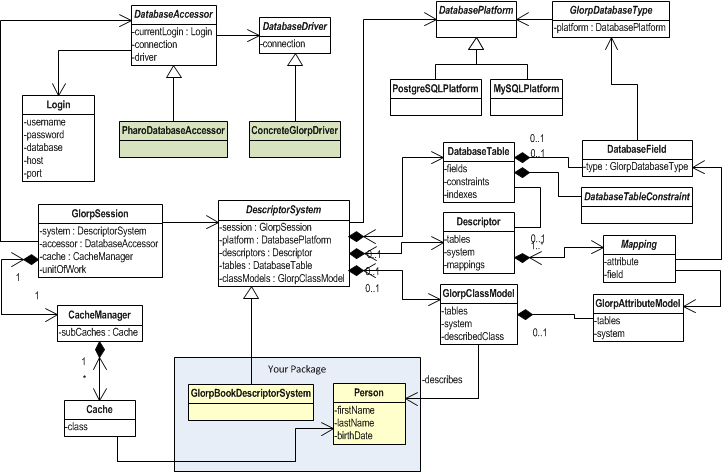
\includegraphics[width=0.72\textwidth]{/Users/ducasse/Workspace/FirstCircle/MyBooks/Bk-Writing/PharoBooks2/Booklet-Glorp/_result/pdf/Chapters/Glorp/figures/Glorp-Model.png}\caption{Glorp objects UML Diagram\label{glorpObjectModel}}\end{center}
\end{figure}

\chapter{Appendix A: Basic Relational Databases Concepts}\section{Tables}
A table is a collection of related data held in a structured format within a database.
It consists of fields (columns), and rows.

In relational databases and flat file databases, a table is a set of data
elements (values) using a model of vertical columns (identifiable by name)
and horizontal rows, the cell being the unit where a row and column intersect.

A table has a specified number of columns, but can have any number of rows.
Each row is identified by one or more values appearing in a particular column
subset. The columns subset which uniquely identifies a row is called the
primary key.
\section{Rows}
In the context of a relational database, a row —also called a \textit{record} or
\textit{tuple}— represents a single, implicitly structured data item in a table.
In simple terms, a database table can be thought of as consisting of rows
and columns or fields. Each row in a table represents a set of related data,
and every row in the table has the same structure.
\section{Columns}
For example, in a table that represents companies, each row would represent a
single company. Columns might represent things like company name,
company street address, whether the company is publicly held, its VAT number,
etc.. In a table that represents the association of employees with departments,
each row would associate one employee with one department.
\section{Constraints}
Constraints make it possible to further restrict the domain of an attribute. For
instance, a constraint can restrict a given integer attribute to values between
1 and 10. Constraints provide one method of implementing business rules in the
database. SQL implements constraint functionality in the form of check
constraints.

Constraints restrict the data that can be stored in relations. These are usually
defined using expressions that result in a boolean value, indicating whether or
not the data satisfies the constraint. Constraints can apply to single
attributes, to a tuple (restricting combinations of attributes) or to an entire
relation.

 Since every attribute has an associated domain, there are constraints (domain
constraints). The two principal rules for the relational model are known as
entity integrity and referential integrity.
\subsection{Primary Key}
A primary key uniquely specifies a tuple within a table. In order for an attribute to be a good primary key it must not repeat. While
natural attributes (attributes used to describe the data being entered) are
sometimes good primary keys, surrogate keys are often used instead.

A surrogate key is an artificial attribute assigned to an object which uniquely
identifies it (for instance, in a table of information about students at a
school they might all be assigned a student ID in order to differentiate them).

The surrogate key has no intrinsic (inherent) meaning, but rather is useful
through its ability to uniquely identify a tuple. Another common occurrence,
especially in regard to N:M cardinality is the composite key. A composite key is
a key made up of two or more attributes within a table that (together) uniquely
identify a record. (For example, in a database relating students, teachers, and
classes. Classes could be uniquely identified by a composite key of their room
number and time slot, since no other class could have exactly the same
combination of attributes. In fact, use of a composite key such as this can be a
form of data verification, albeit a weak one.
\subsection{Foreign Keys}
A foreign key is a field in a relational table that matches
the primary key column of another table. The foreign key can be used to
cross-reference tables. Foreign keys do not need to have unique values in the
referencing relation. Foreign keys effectively use the values of attributes in
the referenced relation to restrict the domain of one or more attributes in the
referencing relation.
\section{Indexes}
An index is one way of providing quicker access to data. Indices can be created
on any combination of attributes on a relation. Queries that filter using those
attributes can find matching tuples randomly using the index, without having to
check each tuple in turn. This is analogous to using the index of a book to go
directly to the page on which the information you are looking for is found, so
that you do not have to read the entire book to find what you are looking for.

Relational databases typically supply multiple indexing techniques, each of
which is optimal for some combination of data distribution, relation size, and
typical access pattern.

Indices are usually not considered part of the database, as they are considered
an implementation detail, though indices are usually maintained by the same
group that maintains the other parts of the database. It should be noted that
use of efficient indexes on both primary and foreign keys can dramatically
improve query performance.
\section{Relations}\subsection{Joins}
A SQL join clause combines records from two or more
tables in a relational database. A JOIN is a means for combining fields from two
tables (or more) by using values common to each

ANSI-standard SQL specifies five types of JOIN: INNER, LEFT OUTER, RIGHT OUTER,
FULL OUTER and CROSS. As a special case, a table (base table, view, or joined
table) can JOIN to itself in a self-join.
\subsection{INNER JOINs}
An inner join requires each record in the two joined tables to
have matching records, and is a commonly used join operation in applications but
should not be assumed to be the best choice in all situations. Inner join
creates a new result table by combining column values of two tables (A and B)
based upon the join-predicate. The query compares each row of A with each row of
B to find all pairs of rows which satisfy the join-predicate. When the
join-predicate is satisfied by matching non-NULL values, column values for each
matched pair of rows of A and B are combined into a result row.

The result of the join can be defined as the outcome of first taking the
Cartesian product (or Cross join) of all records in the tables (combining every
record in table A with every record in table B) and then returning all records
which satisfy the join predicate. Actual SQL implementations normally use other
approaches, such as hash joins or sort-merge joins, since computing the
Cartesian product is slower and would often require a prohibitively large memory
space to store. 
\subsubsection{OUTER JOINs }
The joined table retains each record—even if no other matching record exists. Outer joins subdivide further into left outer
joins, right outer joins, and full outer joins, depending on which table's rows
are retained (left, right, or both).

The result of a left outer join (or simply left join) for tables A and B always
contains all records of the \symbol{34}left\symbol{34} table (A), even if the join-condition does
not find any matching record in the \symbol{34}right\symbol{34} table (B). This means that if the ON
clause matches 0 (zero) records in B (for a given record in A), the join will
still return a row in the result (for that record)—but with NULL in each column
from B. A left outer join returns all the values from an inner join plus all
values in the left table that do not match to the right table, including rows
with NULL (empty) values in the link field.

For example, this allows us to find an employee's department, but still shows
employees that have not been assigned to a department (contrary to the
inner-join example above, where unassigned employees were excluded from the
result).
\section{Data manipulation language (DML) queries}\subsection{SELECT}
A \textcode{SELECT} statement retrieves zero or more rows from one
or more database tables or database views. In most applications, SELECT is the
most commonly used data manipulation language (DML) command. As SQL is a
declarative programming language, SELECT queries specify a result set, but do
not specify how to calculate it. The database translates the query into a \symbol{34}query
plan\symbol{34} which may vary between executions, database versions and database
software. This functionality is called the \symbol{34}query optimizer\symbol{34} as it is
responsible for finding the best possible execution plan for the query, within
applicable constraints.
\subsection{INSERT}
An SQL \textcode{INSERT} statement adds one or more
records to any single table in a relational database.

The number of columns and values must be the same. If a column is not specified,
the default value for the column is used. The values specified (or implied) by
the INSERT statement must satisfy all the applicable constraints (such as
primary keys, CHECK constraints, and NOT NULL constraints). If a syntax error
occurs or if any constraints are violated, the new row is not added to the table
and an error returned instead.
\subsection{UPDATE}
An SQL \textcode{UPDATE} statement changes the data of one or more records in a
table. Either all the rows can be updated, or a subset may be chosen using a
condition.

In some databases, such as PostgreSQL, when a FROM clause is present, what
essentially happens is that the target table is joined to the tables mentioned
in the fromlist, and each output row of the join represents an update operation
for the target table. When using FROM, one should ensure that the join produces
at most one output row for each row to be modified. In other words, a target row
shouldn't join to more than one row from the other table(s). If it does, then
only one of the join rows will be used to update the target row, but which one
will be used is not readily predictable.

Because of this indeterminacy, referencing other tables only within sub-selects
is safer, though often harder to read and slower than using a join.
\subsection{DELETE}
In the database structured query language (SQL), the \textcode{DELETE}
statement removes one or more records from a table. A subset may be defined for
deletion using a condition, otherwise all records are removed.

Any rows that match the WHERE condition will be removed from the table. If the
WHERE clause is omitted, all rows in the table are removed. The DELETE statement
should thus be used with caution.

The DELETE statement does not return any rows; that is, it will not generate a
result set.



% lulu requires an empty page at the end. That's why I'm using
% \backmatter here.
\backmatter

% Index would go here

\end{document}
